\tableofcontents
\section*{Предисловие}
При выполнении данной лабораторной работы было решено использовать 
\href{https://python-control.readthedocs.io/en/0.9.4/}{Python Control Systems Library}.
Данный инструмент является альтернативой Matlab, адаптированной для использования на 
языке Python и предоставляет широкий функционал для анализа и моделирования систем,
а также синтеза регуляторов для управления.

Полный листинг моделирования систем представлен в \href{https://github.com/diuzhevVlad/control-theory-itmo-fall-2023/blob/main/Lab3/Lab3.ipynb}{jupyter notebook} на GitHub.

\pagebreak



\section{Вынужденное движение}
Рассмотрим систему второго порядка в форме В-В:
\begin{equation}
    \ddot{y} + a_1 \dot{y} + a_0 y  = u
\end{equation}
Согласно заданию, выберем три набора корней $(\lambda_1, \lambda_2)$, удовлетворяющих модам из задания (5,6,7)
и найдем небходимые пары коэффициентов $(a_1, a_0)$:
\begin{enumerate}
    \item Нейтральная и пропорциональная времени: $\lambda_1 = 0, \lambda_2 = 0$; $a_1 = 0, a_0 = 0$
    \item Пара консервативных мод: $\lambda_1 = i, \lambda_2 = -i$; $a_1 = 0, a_0 = 1$
    \item Пара усточивых колебательных мод: $\lambda_1 = -1 - i, \lambda_2 = -1 + i$; $a_1 = 2, a_0 = 2$
\end{enumerate}

Проведем моделирование систем (рис. 1-3).

Заметим, что устойчивые системы сходятся к единому поведению в течении переходного процесса.
Неустойчивые или находящиеся на границе устойчивости могут вести себя по разному в зависимости
от подаваемого воздействия.
\begin{figure}[h]
    \centering
    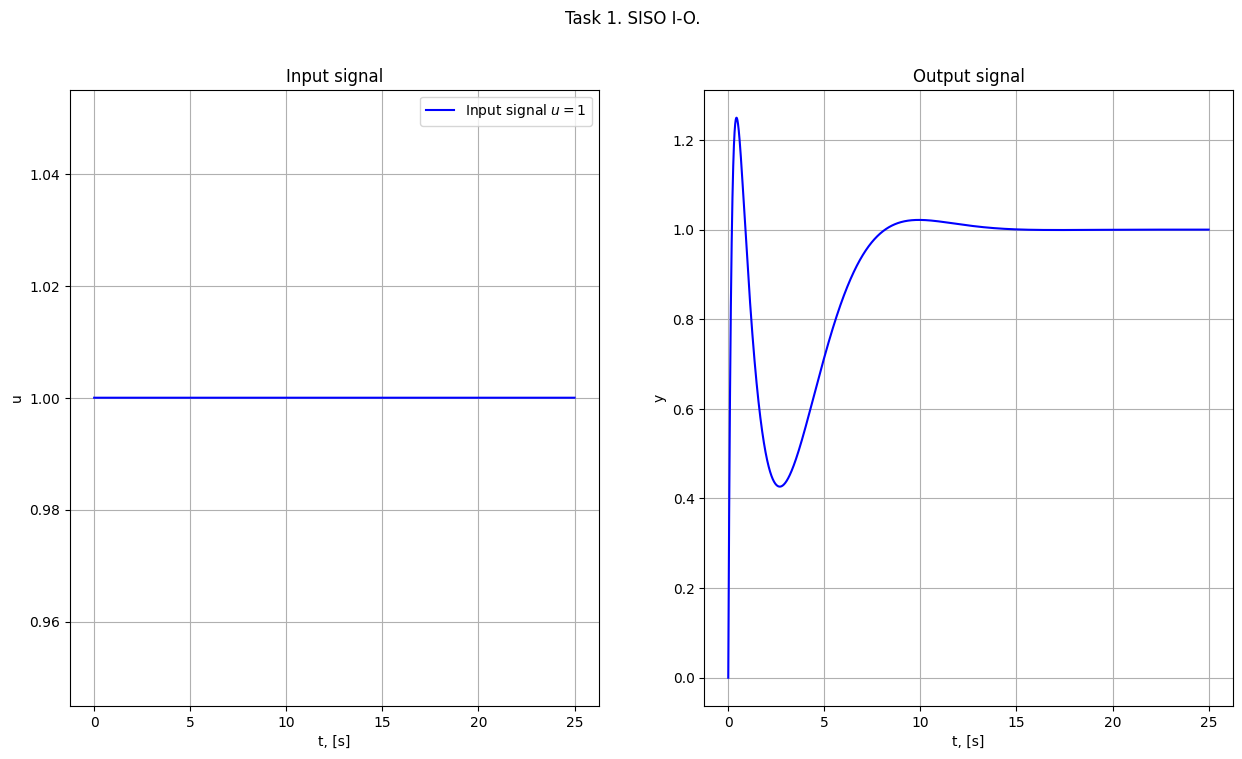
\includegraphics[width=\textwidth]{plot_1_1}
    \caption{\label{fig:The-caption-1}Выходные сигналы системы 1 при различных начальных условиях и входных воздействиях (задание 1)}
\end{figure}
\begin{figure}[]
    \centering
    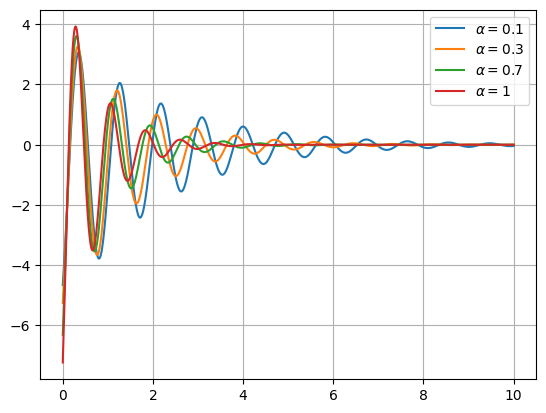
\includegraphics[width=\textwidth]{plot_1_2}
    \caption{\label{fig:The-caption-1}Выходные сигналы системы 2 при различных начальных условиях и входных воздействиях (задание 1)}
\end{figure}
\begin{figure}[]
    \centering
    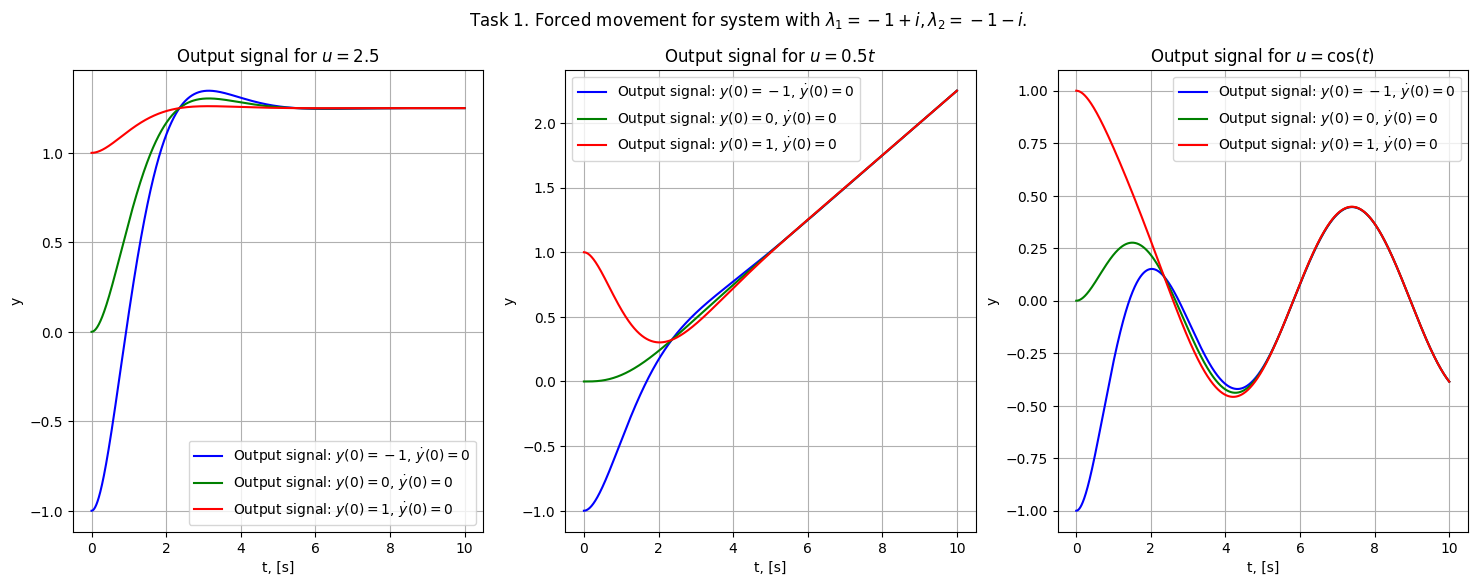
\includegraphics[width=\textwidth]{plot_1_3}
    \caption{\label{fig:The-caption-1}Выходные сигналы системы 3 при различных начальных условиях и входных воздействиях (задание 1)}
\end{figure}
\pagebreak

\section{Качество переходных процессов}
Оценивать качество переходного процесса будем с помощью двух параметров: перерегулирования $(\Delta \sigma)$
и времени переходного процесса $(T_s)$. Определим $T_s$ как время, после которого система не покидает $5\%$ интервал
от установившегося значения. $\Delta \sigma = |\frac{y_{max} - y_{st}}{y_{st}}|$, где 
$y_{st}$ - установившееся значение, $y_{max}$ - максимальное по отклонению значение сигнала.

Рассмотрим систему с передаточной функцией:
\begin{equation}
    W(s) = \frac{1}{(s-\lambda_1)(s-\lambda_2)(s-\lambda_3)}
\end{equation}
Проведем моделирование системы при нулевых начальных условиях с функцией $1(t)$ в качестве входного воздействия (рис. 4-6).

\begin{figure}[h]
    \centering
    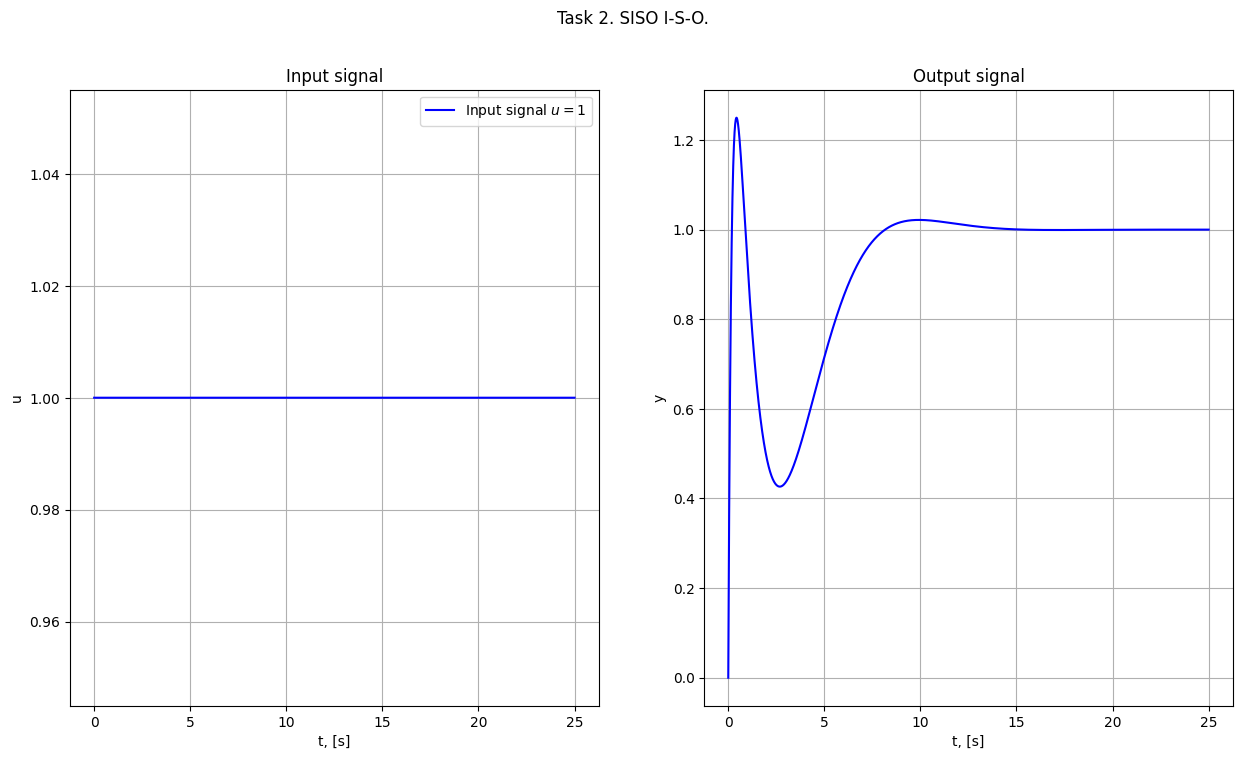
\includegraphics[width=\textwidth]{plot_2_1}
    \caption{\label{fig:The-caption-1} Исследование влияния чисто действительных корней на качество переходного процесса (задание 2)}
\end{figure}
Заметим, что при малом по модулю значению полюсов, можно достичь низкого перерегулирования и времени переходного процесса. При 
увеличении модуля полюсов перерегулирование растет, как и время переходного процесса. 
При еще больших значениях, перерегулирование вырастает еще больше, однако время сзодимости снижается.
\pagebreak
\begin{figure}[h]
    \centering
    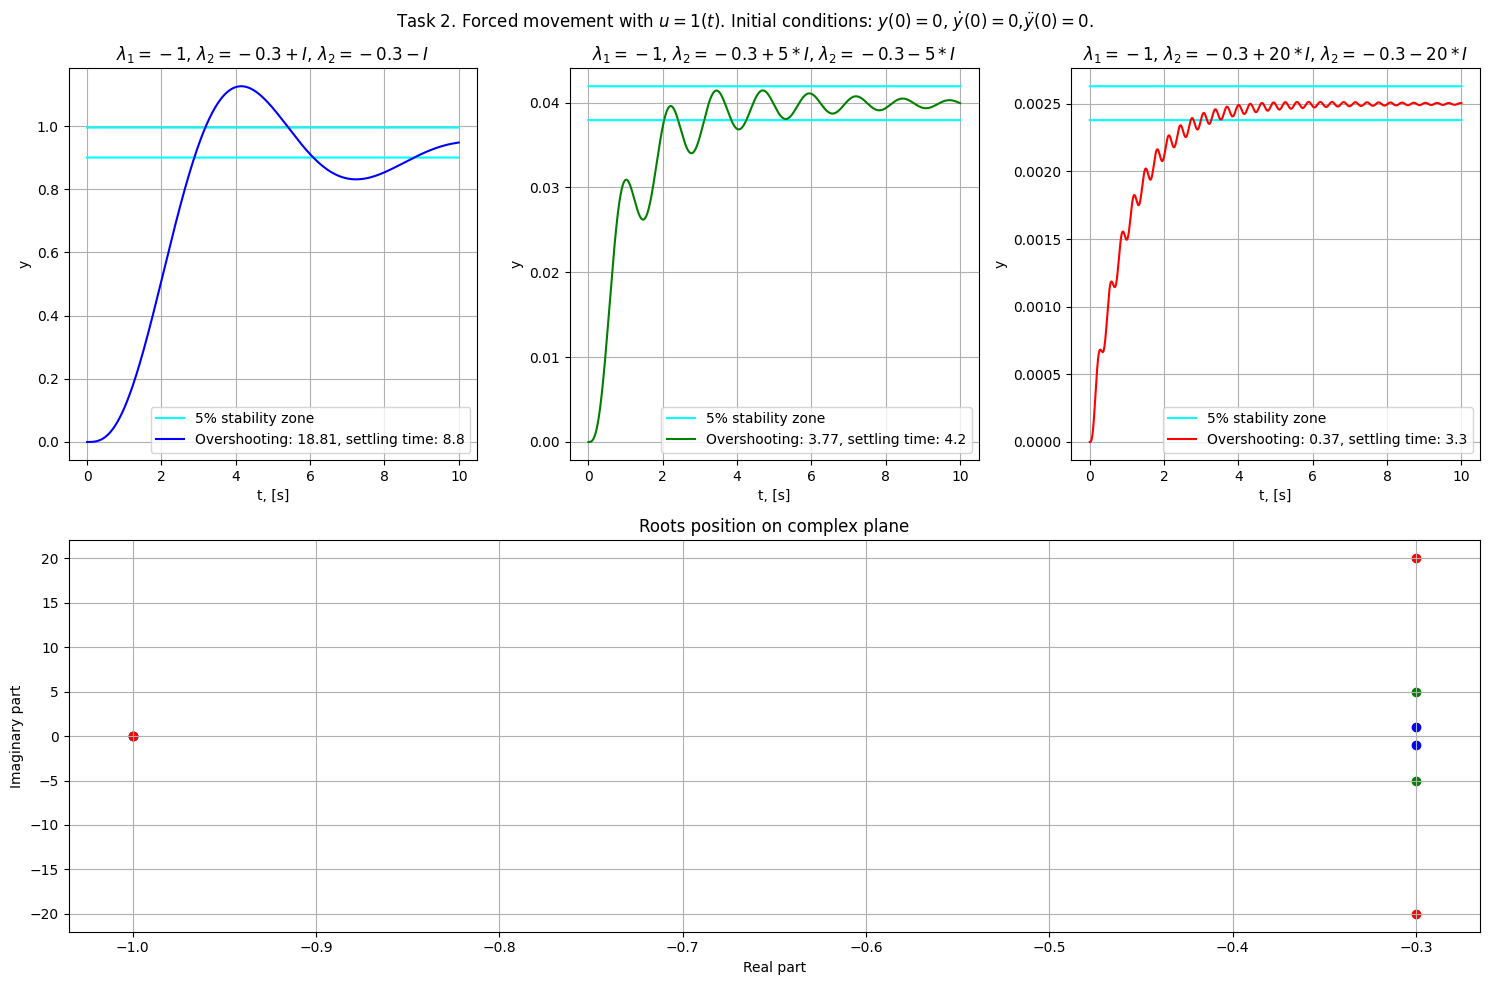
\includegraphics[width=\textwidth]{plot_2_2}
    \caption{\label{fig:The-caption-1} Исследование влияния величины мнимой части корней на качество переходного процесса (задание 2)}
\end{figure}

Увеличение мнимой части полюсов ведет к росту времени переходного процесса и перерегулирования.
\pagebreak
\begin{figure}[h]
    \centering
    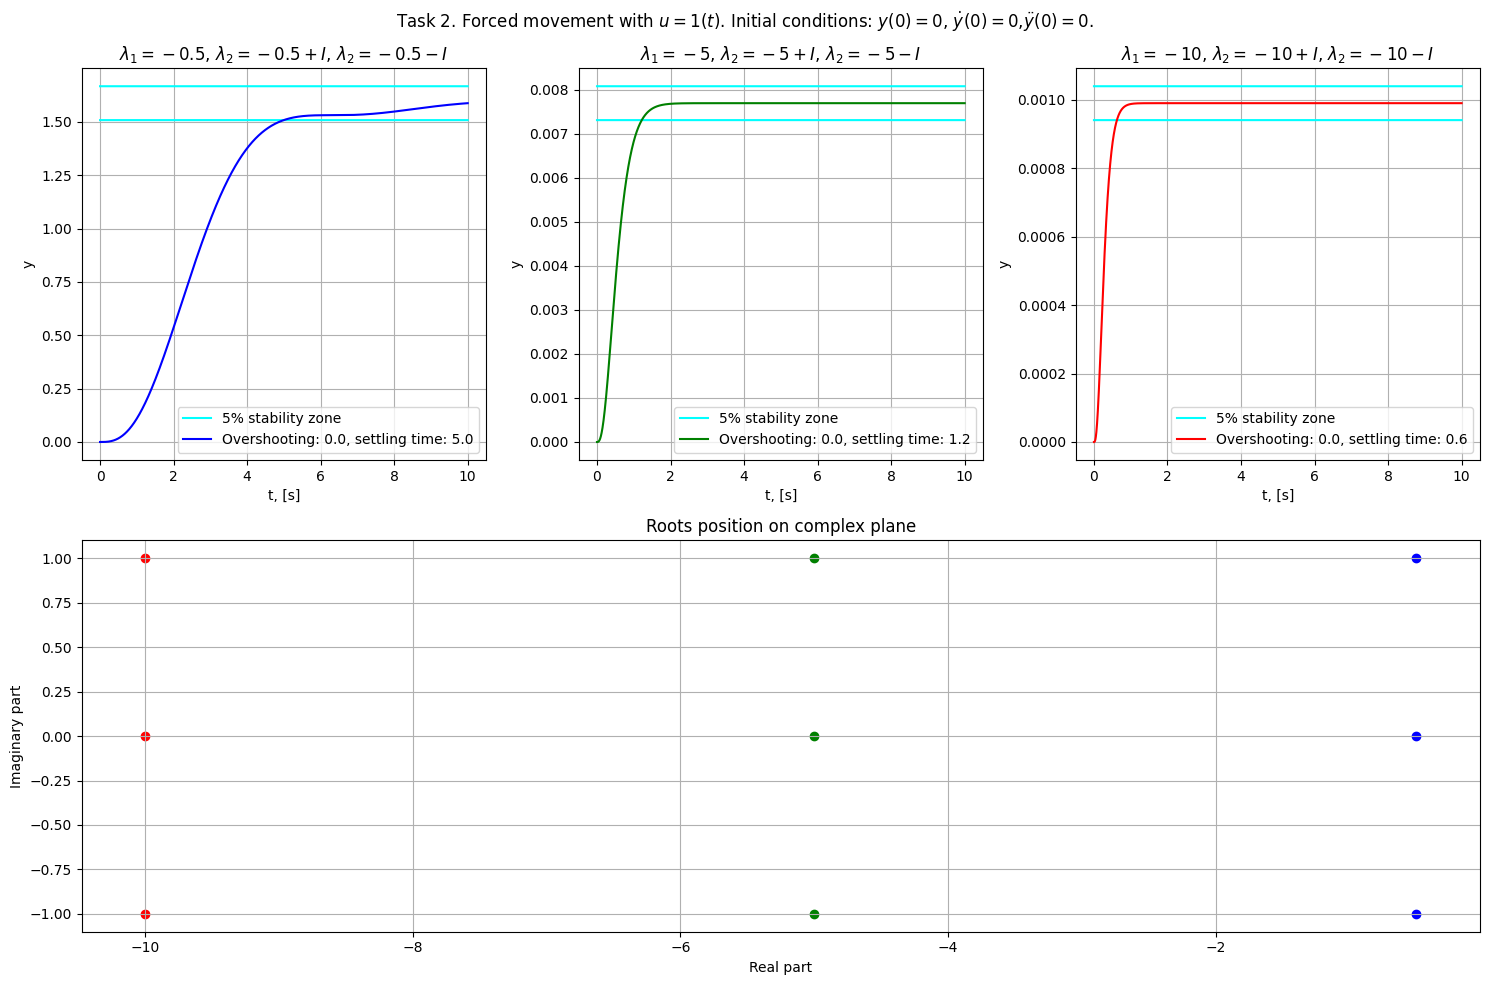
\includegraphics[width=\textwidth]{plot_2_3}
    \caption{\label{fig:The-caption-1} Исследование влияния действительной части корней на качество переходного процесса (задание 2)}
\end{figure}

Можем заметить схожее поведение с рис. 4. Мнимая часть добавляет колебательный характер системе.
\pagebreak

\section{Свертка, как произведение образов Лапласа}

Рассмотрим систему вида:
\begin{equation}
    y(t) = W(s)[u(t)],
    W(s) = \frac{6}{(s+2)^4}, u(t)=\cos{2t} - 2\cos{3t}
\end{equation}
Можем записать:
\begin{equation*}
    y(t) = \int_{0}^{t}w(t - \tau)u(\tau)d\tau, w(t) = \mathcal{L}^{-1}(W(s))
\end{equation*}
или:
\begin{equation*}
    y(t) = Y(s)[\delta(t)], Y(s)=W(s)\mathcal{L}(u(t))
\end{equation*}

Проверим эквивалентность, данных подходов:
\begin{figure}[h]
    \centering
    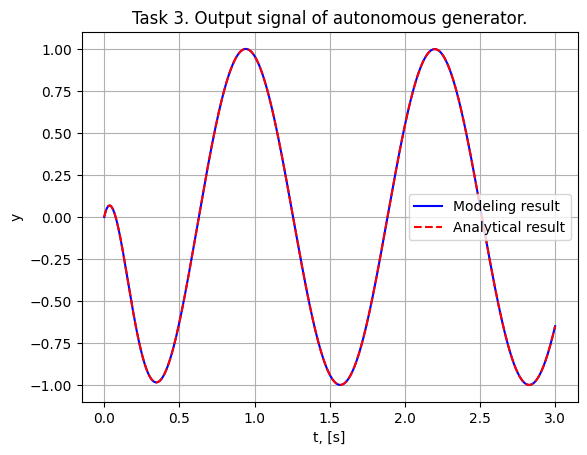
\includegraphics[width=\textwidth]{plot_3_1}
    \caption{\label{fig:The-caption-1} Сравнение графиков стандартного моделирования процесса, свертки и моделирования в импульсном режиме (задание 3)}
\end{figure}

Как видим, графики совпадают.

\pagebreak

\section{Выводы}
В ходе данной лабораторной работы удалось изучить поведение систем разных типов устойчивости при 
вынужденном движении с различными начальными условиями. Также было показано влияние полюсов передаточной функции
на характер и параметры переходного процесса. Кроме того, удалось продемонстрировать свойства преобразования Лапласа
 (в частности, его связь со сверткой функций).
\begin{enumerate}
    \item Устойчивые системы сходятся к единой траектории при вынужденном движении. Поведение неустойчивых систем предсказать сложно,
 однако можно заметить, что колебательный характер остается.
    \item  Снижение действительной части полюсов передаточной функции ведет к более быстрому
 схождению системы, однако увеличивает перерегулирование. Мнимая часть придает колебательный характер системе,
 что негативно сказывается на параметрах переходного процесса. Можно заметить, что наибольшее влияние на поведение
 системы оказывает корень с наибольшем действительной частью.
    \item Наглядно подтвердилось утверждение о том, что результат применения преобразования Лапласа к свертке функций 
 равен произведению образов Лапласа данных функций.
\end{enumerate}
\pagebreak